\documentclass[journal,12pt,twocolumn]{IEEEtran}

\usepackage{enumitem}
\usepackage{amsmath}
\usepackage{amssymb}
\usepackage{gensymb}
\usepackage{graphicx}
\usepackage{txfonts}         
\usepackage{listings}
\usepackage{lstautogobble}
\usepackage{mathtools}
\usepackage{bm}
\usepackage{hyperref}
\usepackage{polynom}
\usepackage{capt-of}
\newcommand{\solution}{\noindent \textbf{Solution: }}
\providecommand{\pr}[1]{\ensuremath{\Pr\left(#1\right)}}
\providecommand{\brak}[1]{\ensuremath{\left(#1\right)}}
\providecommand{\cbrak}[1]{\ensuremath{\left\{#1\right\}}}
\providecommand{\sbrak}[1]{\ensuremath{\left[#1\right]}}
\providecommand{\mean}[1]{E\left[ #1 \right]}
\providecommand{\var}[1]{\mathrm{Var}\left[ #1 \right]}
\providecommand{\der}[1]{\mathrm{d} #1}
\providecommand{\gauss}[2]{\mathcal{N}\ensuremath{\left(#1,#2\right)}}
\providecommand{\mbf}{\mathbf}
\providecommand{\abs}[1]{\left\vert#1\right\vert}
\providecommand{\norm}[1]{\left\lVert#1\right\rVert}
\providecommand{\z}[1]{{\mathcal{Z}}\{#1\}}
\providecommand{\ztrans}{\overset{\mathcal{Z}}{ \rightleftharpoons}}

\providecommand{\parder}[2]{\frac{\partial}{\partial #2} \brak{#1}}

\let\StandardTheFigure\thefigure
\let\vec\mathbf

\numberwithin{equation}{section}
\renewcommand{\thefigure}{\theenumi}
\renewcommand\thesection{\arabic{section}}

\newcommand{\myvec}[1]{\ensuremath{\begin{pmatrix}#1\end{pmatrix}}}
\newcommand{\mydet}[1]{\ensuremath{\begin{vmatrix}#1\end{vmatrix}}}
\newcommand{\define}{\stackrel{\triangle}{=}}

\DeclareMathOperator*{\argmin}{arg\,min}
\DeclareMathOperator*{\argmax}{arg\,max}


\lstset {
	frame=single, 
	breaklines=true,
	columns=fullflexible,
	autogobble=true
}             
   


\begin{document}
                             
\title{ EE3900: Linear Systems and Signal Processing \\ {Assignment-2}}
\author{Aakash Kamuju\\ \normalsize AI21BTECH11001 }
 \maketitle 
 \begin{abstract}
 This document contains solution to Assignment-2 [ Question 2.1(b) from Discrete-Time Signal Processing by Alan V. Oppenheim and Ronald W. Schafer]
 \end{abstract}
 \section*{Linear Time Invariant System}
\begin{enumerate}[label=\arabic*]
\item Let $x\sbrak{n} = \delta\sbrak{n} + 2\delta\sbrak{n-1}-\delta\sbrak{n-3}$ and
$h\sbrak{n} =2\delta\sbrak{n+1}+2\delta\sbrak{n-1} $.\\
Compute and plot convolution of $y_2\sbrak{n}$\\ $y_2\sbrak{n} = x\sbrak{n+2}*h\sbrak{n}$\\
\solution \\
\begin{align}
\delta\sbrak{n-a}=
\begin{cases}
1 & n=a\\
0 & otherwise
\end{cases}
\end{align}
$x\sbrak{n+2} = \cbrak{1,2,0,-1}$\\
\begin{figure}[!ht]
\centering
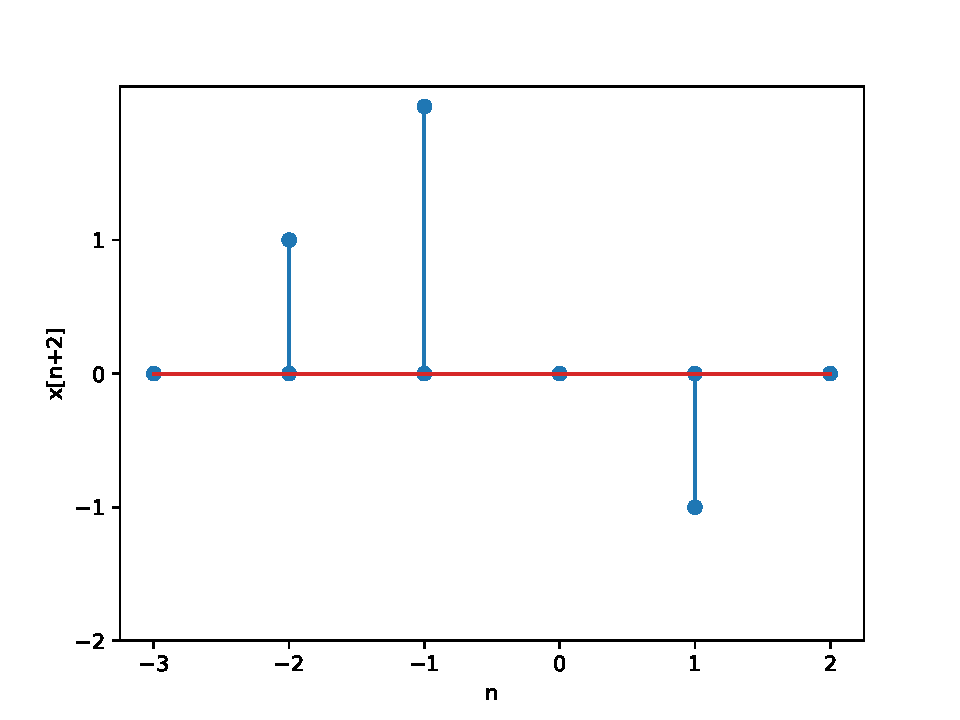
\includegraphics[width=\columnwidth]{./figs/x[n+2]}
\label{fig:x[n+2]}
\end{figure}
$h\sbrak{n} = \cbrak{2,0,2}$
\begin{figure}[!ht]
\centering
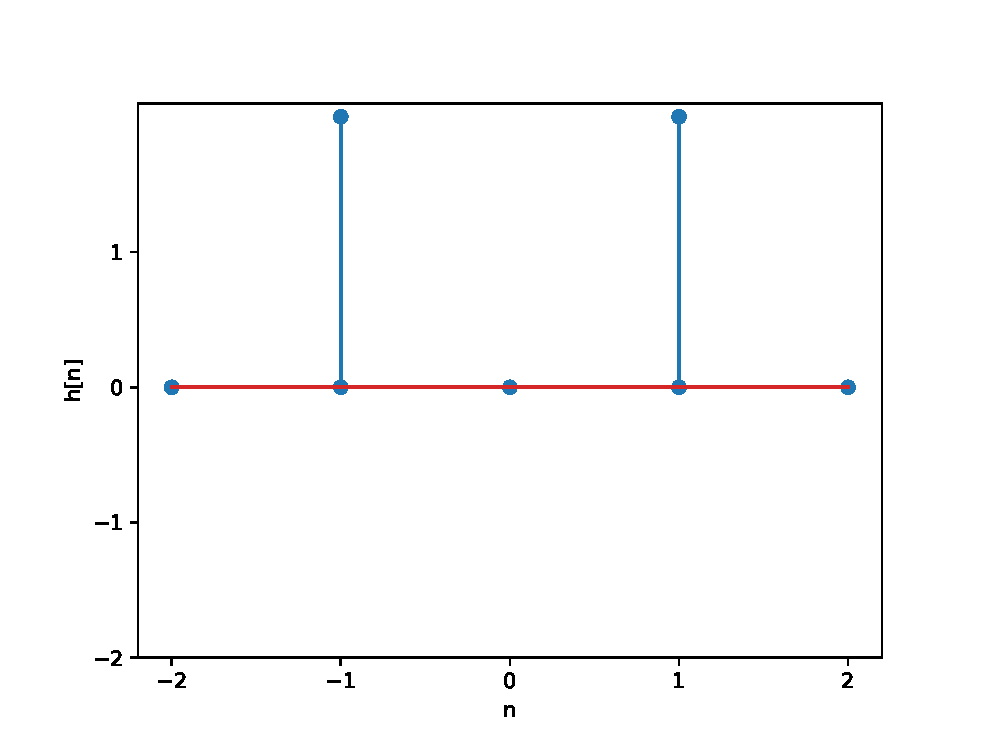
\includegraphics[width=\columnwidth]{./figs/h[n]}
\label{fig:h[n]}
\end{figure}
\begin{align}
\vec{y}&=\myvec{1 & 0&0\\ 2& 1&0\\ 0& 2&1\\-1 & 0&2\\0 & -1&0\\0& 0&-1\\}\myvec{2 \\ 0 \\2}
&=\myvec{2\\4\\2\\2\\0\\-2}\\
\end{align}
So $y\sbrak{n}=\cbrak{2,4,2,2,0,-2}$\\
Plot of convolution is 
\begin{figure}[!ht]
\centering
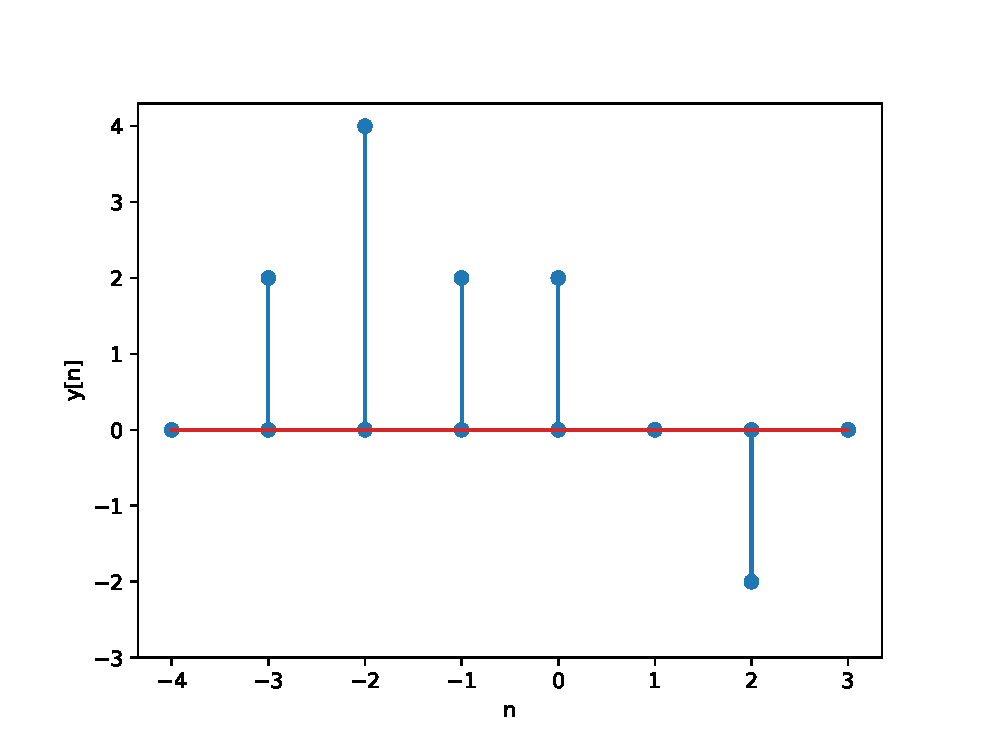
\includegraphics[width=\columnwidth]{./figs/y[n]}
\label{fig:y[n]}
\end{figure}
\end{enumerate} 
 \end{document}
